%%%%%%%%%%%%%%%%%%%%%%%%%%%%%%%%%%%%%%%%%
% Short Sectioned Assignment
% LaTeX Template
% Version 1.0 (5/5/12)
%
% This template has been downloaded from:
% http://www.LaTeXTemplates.com
%
% Original author:
% Frits Wenneker (http://www.howtotex.com)
%
% License:
% CC BY-NC-SA 3.0 (http://creativecommons.org/licenses/by-nc-sa/3.0/)
%
%%%%%%%%%%%%%%%%%%%%%%%%%%%%%%%%%%%%%%%%%

%----------------------------------------------------------------------------------------
%	PACKAGES AND OTHER DOCUMENT CONFIGURATIONS
%----------------------------------------------------------------------------------------

\documentclass[paper=a4, fontsize=11pt]{scrartcl} % A4 paper and 11pt font size
\usepackage[T1]{fontenc}
\usepackage[utf8]{inputenc} %æ,ø,å
\usepackage[english]{babel} % English language/hyphenation
\usepackage{amsmath,amsfonts,amsthm} % Math packages
\usepackage{listings}

\usepackage[tocflat]{tocstyle}
\addto\captionsenglish{% Replace "english" with the language you use
  \renewcommand{\contentsname}%
    {Innholdsfortegnelse}%
}

\usepackage{sectsty} % Allows customizing section commands
\allsectionsfont{\centering \normalfont\scshape} % Make all sections centered, the default font and small caps

\usepackage{fancyhdr} % Custom headers and footers
\usepackage{placeins} %Floatbarrier

\usepackage{graphicx} %package to manage images
\pagestyle{fancyplain} % Makes all pages in the document conform to the custom headers and footers
\fancyhead{} % No page header - if you want one, create it in the same way as the footers below
\fancyfoot[L]{} % Empty left footer
\fancyfoot[C]{} % Empty center footer
\fancyfoot[R]{\thepage} % Page numbering for right footer
\renewcommand{\headrulewidth}{0pt} % Remove header underlines
\renewcommand{\footrulewidth}{0pt} % Remove footer underlines
\setlength{\headheight}{13.6pt} % Customize the height of the header

\numberwithin{equation}{section} % Number equations within sections (i.e. 1.1, 1.2, 2.1, 2.2 instead of 1, 2, 3, 4)
\numberwithin{figure}{section} % Number figures within sections (i.e. 1.1, 1.2, 2.1, 2.2 instead of 1, 2, 3, 4)
\numberwithin{table}{section} % Number tables within sections (i.e. 1.1, 1.2, 2.1, 2.2 instead of 1, 2, 3, 4)

\setlength\parindent{0pt} % Removes all indentation from paragraphs - comment this line for an assignment with lots of text

%----------------------------------------------------------------------------------------
%	TITLE SECTION
%----------------------------------------------------------------------------------------

\newcommand{\horrule}[1]{\rule{\linewidth}{#1}} % Create horizontal rule command with 1 argument of height

\title{	
\normalfont \normalsize 
\textsc{Universitetet i Oslo, Fysisk Institutt \\
										FYS3150, Prosjekt 5} \\ [25pt] % Your university, school and/or department name(s)
\horrule{0.5pt} \\[0.4cm] % Thin top horizontal rule
\huge Molekylærdynamikk \\ % The assignment title
\horrule{2pt} \\[0.5cm] % Thick bottom horizontal rule
}

\author{Live Wang Jensen} % Your name

\date{\normalsize\today} % Today's date or a custom date

\begin{document}

\maketitle 
\begin{abstract}
Målet med dette prosjektet er å implementere en algoritme som bruker molekylærdynamikk slik at vi kan studere ulike termodynamiske egenskaper til grunnstoffet argon.  Atomene i systemet vårt er ordnet i en kubisk flatesentrerte gitterstruktur, som er den strukturen argon har som fast stoff. Vi har sett på et system med 500 atomer, og simulert systemets tidsutvikling ved ulike initialtemperaturer. I tillegg har vi sett på ulike termodynamiske størrelser som potensiell og kinetisk energi, temperaturutvikling og diffusjonskonstant. Ved å plotte diffusjonskonstanten som funksjon av temperatur, fant vi ut at systemets smeltevarme lå på DKFJSKJFH Kelvin.

\end{abstract}

\tableofcontents


\section{Introduksjon}
Molekylærdynamikk, eller MD, er en numerisk metode som brukes for å kunne beregne ulike fysiske størrelser. Dette gjøres gjerne gjennom datasimulasjon av bevegelsen til atomer. Det finnes flere ulike MD algoritmer, den enkleste av dem bruker Newtonsk fysikk og ser på atomene som punktpartikler. MD er en svært nyttig metode som brukes innen nesten alle vitenskapelige fagfelt, fra biokjemi og materialteknologi til nanoteknologi og biofysikk. Slike simuleringer brukes blant annet til å studere oppførselen til systemer som ikke kan observeres direkte gjennom eksperimenter, som for eksempel vekst av tynnfilmer. Innenfor biofysikken bruker man ofte MD til å raffinere tredimensjonale proteinstrukturer og andre makromolekyler ut ifra eksperimentelle data hentet fra NMR spektroskopi. MD kan også brukes til å undersøke fysiske egenskaper i nanoteknologiske apparater som ennå ikke har blitt produsert. 
\\

I denne oppgaven skal vi se nærmere på grunnstoffet argon. Vi skal gradvis bygge opp en kode som til slutt gjør oss i stand til å simulere ulike egenskaper ved argon ved bruk av molekylærdynamikk. Vi starter med å se på argons gitterstruktur og hvordan denne kan implementeres i koden vår. Dette gjør slik at atomene i systemet vårt plasseres ordnet, og ikke tilfeldig inne i enhetscellen. Videre innfører vi periodiske grensebetingelser, som fører til at vi får et lukket system hvor den totale energien er konstant. Vi skal bruke Lennard-Jones potensialet til å beregne kraften som virker mellom atomene. I tillegg skal vi se nærmere på andre fysiske størrelser som kinetisk og potensiell energi, temperatur og diffusjonskonstant. Systemet vårt består av 500 atomer, og vi skal bruke programmet Ovito til å se på hvordan disse vil oppføre seg som funksjon av tid ved ulike initialtemperaturer. Dette kan brukes som et røft estimat til å finne systemets smeltepunkt. Et mer nøyaktig estimat finner vi ved å se på diffusjonskonstanten som funksjon av temperatur.


\section{Teori og implementasjon}

\subsection{Gitterstruktur}
Gitteret vårt består at \textit{enhetsceller}, en gruppe med atomer. Større systemer vil altså bestå av flere enhetsceller etter hverandre. Argon har en kubisk flatesentrert gitterstruktur, også kalt FCC, se figur \ref{fcc}. 

\FloatBarrier
\begin{figure}[!ht]
 \centering
 \includegraphics[scale=0.3]{fcc.png}
 \caption{To mulige fremstillinger av gitterstrukturen FCC.}
 \label{fcc}
 \end{figure}
 \FloatBarrier

Én slik FCC celle har størrelsen $b$ Ångstrøm, hvor $b$ er gitterkonstanten. Vi bruker $b$ = 5.26 Ångstrøm, som er den vanlige cellestørrelsen i Argon krystallen. Hver celle består av fire atomer med koordinatene
\begin{equation}
\textbf{r}_1 = 0 \hat{i} + 0 \hat{j} + 0 \hat{k}
\end{equation}
\begin{equation}
\textbf{r}_2 = \frac{b}{2} \hat{i} + \frac{b}{2} \hat{j} + 0 \hat{k}
\end{equation}
\begin{equation}
\textbf{r}_3 = 0 \hat{i} + \frac{b}{2} \hat{j} + \frac{b}{2} \hat{k}
\end{equation}
\begin{equation}
\textbf{r}_4 = \frac{b}{2} \hat{i} + 0 \hat{j} + \frac{b}{2} \hat{k}
\end{equation}

Vi kan nå lage $N_x \times N_y \times N_z$ slike enhetsceller ved siden av hverandre for å danne et større system, hvor origo til enhetscelle ($i,j,k$) er 
\begin{equation}
\mathbf{R}_{i,j,k} = i \hat{\mathbf{u}}_1 + j \hat{\mathbf{u}}_2 + k \hat{\mathbf{u}}_3,
\end{equation}

hvor $i=0,1,..., N_x-1, j=0,1,..., N_y-1$, og $k=0,1,..., N_z-1$. Enhetsvektorene til enhetscellene skaleres med gitterkonstanten $b$ slik at
\begin{align}
	\hat{\mathbf{u}}_1 = b\hat{\mathbf{i}}, \quad \hat{\mathbf{u}}_2 = b\hat{\mathbf{j}}, \quad \hat{\mathbf{u}}_3 = b\hat{\mathbf{k}}.
\end{align}

Siden gitterkonstanten $b$ = 5.26 Ångstrøm, og vi har fire atomer per celle, ender vi opp med en tetthet på $\rho = m/V = 4m_{Ar}/b^3 = 1822,8 kg/m^3$.




\subsection{Periodiske grensebetingelser}
Vi bruker såkalte \textbf{periodiske grensebetingelser} når vi simulerer systemet vårt. Når vi simulerer fysiske systemer på datamaskinen, vil disse være begrenset av maskinens kapasitet. Typiske MD simuleringer inneholder ofte flere millioner atomer på et område mindre enn én kubikkmikrometer. Vi kan komme unna det som skjer i enden av denne kuben ved å bruke periodiske grensebetingelser. På denne måten kan vi simulere store (uendelige) systemer ved en enkelt celle. Når et atom beveger seg forbi veggen på den ene siden, vil den dukke opp igjen på motsatt vegg med samme hastighet, se figur \ref{per}. Store systemer består at et uendelig antall slike enhetsceller, hvor én av disse er vår originale simulering, mens resten er kopier, eller \textit{bilder}, av denne. I tre dimensjoner vil vi altså ha én original celle, med 26 naboer, som er kopier av denne. Vi trenger derfor kun å simulere hva som skjer i den originale enhetscellen, og dette sparer oss enormt med beregningstid -og krefter. Dette kan gjøres ved den enkle algoritmen

\begin{lstlisting}
if (periodic_x) then
  if (x <  -x_size * 0.5) x = x + x_size
  if (x >=  x_size * 0.5) x = x - x_size
end if
\end{lstlisting}

hvor \texttt{x$\_$size} er lengden på boksen i én retning, og \texttt{x} er posisjonen til atomet i denne retningen. I tillegg må avstanden mellom atomene følge \textit{minimum image} kriteriet

\begin{lstlisting}
if (periodic_x) then
  dx = x(j) - x(i)
  if (dx <= -x_size * 0.5) dx = dx + x_size
  if (dx >  x_size * 0.5) dx = dx - x_size
endif
\end{lstlisting}

hvor \texttt{dx} er avstanden mellom atom $i$ og $j$. Vi vet at i tre dimensjoner så vil hvert atom eksistere 27 ganger, en gang i originalcellen og 26 ganger i nabocellene. Når vi beregner kraften som virker mellom atom $i$ og $j$, velger vi altså den kopien av atom $j$ som ligger \textit{nærmest} atom $i$.  Siden vi jobber i tre dimensjoner, må vi gjøre samme prosedyre i y -og z-retning. De eneste kreftene som virker i systemet vårt er indre krefter, slik at den totale energien er konstant. De periodiske grensebetingelsene fører til at systemet ikke kan utveksle atomer med miljøet rundt, som betyr at vi kan kalle dette for et \textit{mikrokanonisk ensemble}. 


\FloatBarrier
\begin{figure}[!ht]
 \centering
 \includegraphics[scale=0.3]{periodic.png}
 \caption{Periodiske grensebetingelser i 2D. Her har vi én original enhetscelle, og åtte kopier av denne.}
 \label{per}
 \end{figure}
 \FloatBarrier
 
 
\subsection{Lennard-Jones potensialet}
Vi kommer til å bruke Lennard-Jones potensialet til å beregne energien mellom to atomer $i$ og $j$

\begin{equation}
U(r_{ij}) = 4\epsilon\left[\left(\frac{\sigma}{r_{ij}}\right)^{12} - \left(\frac{\sigma}{r_{ij}}\right)^6\right],
\end{equation}

hvor $r_{ij} = \vert\mathbf{r}_i - \mathbf{r}_j\vert$  er avstanden mellom atom $i$ og atom $j$, $\epsilon$ er dybden på potensialbrønnen (med enhet energi) og $\sigma$ er avstanden når potensialet er null.\\

Lennard-Jones potensialet er vanlig å bruke når vi skal beskrive kreftene som virker mellom to nøytrale atomer eller molekyler. Argon er en edelgass og vil derfor ikke danne kovalente bindinger mellom atomene. I ligning (2.7) ser vi et ledd $r^{-12}$. Dette leddet beskriver de frastøtende kreftene, som kommer av at atomene frastøter hverandre når avstanden mellom dem er liten, siden deres elektronbaner vil overlappe. Dette kalles den steriske effekten, som fører til at energien øker brått når avstanden blir mindre. Dette illustreres i figur \ref{LJ}. Leddet $r^{-6}$ beskriver den tiltrekkende kraften, som virker ved lengre avstander. Her virker van der Waals krefter, som er en relativt svak kraft, i forholdt til kovalente bindinger.

\FloatBarrier
\begin{figure}[!ht]
 \centering
 \includegraphics[scale=0.4]{LJ.png}
 \caption{Graf som viser styrken på potensialet som funksjon av avstand mellom atomene. $r_m$ er avstanden når potensialet har verdien $-\epsilon$.}
 \label{LJ}
 \end{figure}
 \FloatBarrier


Siden vi jobber med argon, bruker vi 

\begin{equation}
	\frac{\epsilon}{k_B} = 119.8\mathrm{K}, \quad \sigma=3.405 \mathrm{Angstrom}.
\end{equation}

I dette prosjektet brukes såkalte MD enheter. Definisjonen av disse finnes i Appendix A. Potensialet gitt ovenfor gir oss termodynamiske størrelser som stemmer godt med argons eksperimentelle dataer ved ekvilibrium. Systemets tilstandsligning er gitt ved van der Waals ligning. Systemets totale potensielle energi $V$ finner vi ved å summe over alle atompar, hvor vi teller hvert par kun én gang
\begin{equation}
V = \sum_{i>j} U(r_{ij})
\end{equation}

Kraften finner vi ved
\begin{equation}
\textbf{F}(r_{ij}) = - \nabla U(r_{ij}).
\end{equation}

x-komponenten av kraften blir da
\begin{equation}
F_x (r_{ij}) = -\frac{\partial U}{\partial r_{ij}} \frac{\partial r_{ij}}{\partial x_{ij}}.
\end{equation}
y -og z-komponenten finner vi på samme måte. Ved å bruke at $r = \sqrt{x^2 + y^2 + z^2}$, kan vi  derivere dette uttrykket analytisk, slik at 

\begin{equation}
\frac{\partial U}{\partial r_{ij}} = 4 \epsilon \left[ -12 \left( \frac{\sigma^{12}}{r_{ij}^{13}} \right) + 6 \left( \frac{\sigma^6}{r_{ij}^7} \right) \right]
\end{equation}

og 
\begin{equation}
\frac{\partial r_{ij}}{\partial x_{ij}} = \frac{x_{ij}}{r_{ij}},
\end{equation}
slik at 

\begin{equation}
F_x (r_{ij}) = - 4 \epsilon \left[ -12 \left( \frac{\sigma^{12}}{r_{ij}^{13}} \right) + 6 \left( \frac{\sigma^6}{r_{ij}^7} \right) \right] \cdot \frac{x_{ij}}{r_{ij}}.
\end{equation}

Tilsvarende kan gjøres for $F_y(r_{ij})$ og $F_z(r_{ij})$. Når vi implementerer dette i koden vår, bruker vi \textbf{Velocity Verlet} metoden som integrator. Vi finner altså atomenes hastighet og posisjon ved å bruke at 

\[ \vec{v}(t + dt/2) = \vec{v}(t) + \frac{\vec{F}(t)}{m}\frac{dt}{2} \]
\[\vec{r}(t + dt) = \vec{r}(t) + \vec{v}(t + dt/2)dt \]
\[\vec{v}(t + dt) = \vec{v}(t + dt/2) + \frac{\vec{F}(t + dt)}{m} \frac{dt}{2} \]

hvor $dt$ er tidssteget vårt.


\subsection{Kinetisk energi, temperatur og diffusjonskonstanten}
Vi har også beregnet flere ulike fysiske størrelser som kinetisk energi, total energi, temperatur og diffusjonskonstant for å kunne se hvordan systemet utvikler seg ved ulike initialtemperaturer. 

Systemets kinetiske energi er 
\begin{equation}
E_k = \sum_{i=1}^{N_{atomer}} \frac{1}{2}m_iv_i^2
\end{equation}
hvor $m_i$ og $v_i$ er massen og hastigheten til atom nummer $i$. Den potensielle energien er gitt i ligning (2.9), og vi finner den totale energien ved å addere den kinetiske og den potensielle energien. 

\begin{equation}
E_{tot} =  E_k + V
\end{equation}
Vi vet at denne summen må være konstant, siden vi jobber med et mikrokanonisk system. I tillegg skal den totale bevegelsesmengden i systemet være null. Dette er derfor en god måte å teste om programmet virker som det skal.

Vi kan kalkulere et estimat for temperaturen ved hjelp av ekvipartisjonsteoremet 
\begin{equation}
\langle E_k \rangle = \frac{3}{2}N_{atomer} k_B T
\end{equation}
som kan brukes til å definere den \textit{momentane} temperaturen

\begin{equation}
T = \frac{2}{3}\frac{E_k}{N_{atomer} k_B}
\end{equation}

Til slutt kan vi finne diffusjonskonstanten ved å bruke Einstein relasjonen som sier at

\begin{equation}
\langle r^2(t) \rangle = 6 D t
\end{equation}

hvor $D$ er diffusjonskonstanten, $t$ er tiden og

\begin{equation}
r_i^2 (t) = | \textbf{r}_i (t) - \textbf{r}_i (0) |^2
\end{equation} 
hvor $\textbf{r}_i (t)$ er posisjonen til atom $i$ ved tiden $t$. Ved å øke temperaturen, vil systemet bli mer og mer kaotisk. Ved en viss temperatur vil vi miste krystallstrukturen, vi kaller dette for systemets smeltepunkt. Diffusjonskonstanten $D$ gir oss en estimat på temperaturen ved smeltepunktet. Vi vet at $D$ vil være omtrent null når systemet er i fast form, mens den vil øke kraftig ved smeltepunktet.\\



\subsection{Kodens struktur}
Koden som er brukt i dette prosjektet er objekt orientert, og bygger på koden skrevet av Anders Hafreager [6]. Figur \ref{flow} viser kodens flytskjema. Koden består av en rekke nøstede funksjoner som avhenger av hverandre. Aller først starter vi med å initialisere systemet vårt, ved å bestemme antall celler i gitteret, den initielle temperaturen og gitterkonstanten, som bestemmer systemets tetthet. Deretter konverteres enhetene i klassen \texttt{unitconverter.cpp}, slik at ulike fysiske størrelser som masse, lengde og energi har en enhet som er tilpasset systemet vi jobber med. Deretter setter vi opp selve gitteret ved å plassere partiklene i en tredimensjonal kubisk flatesentrert gitterstruktur, akkurat som i argons krystallstruktur. Det betyr at vi har ett atom i hvert hjørne, og ett atom på hver flate. Hvert atom får en tilfeldig initialhastiget bestemt av Boltzmanns fordelingslov som funksjon av initialtemperaturen, slik at 

\begin{equation}
P(v_i)dv_i = \left(\frac{m}{2\pi k_B T} \right)^{1/2} exp \left(- \frac{mv_i^2}{2k_B T} \right)dv_i
\end{equation}

hvor $m$ er atomets masse, $k_B$ er Boltzmanns konstant og $T$ er temperaturen. Dette er en normalfordeling med null i gjennomsnitt og standardavvik $\sigma = \sqrt{k_B T/m}$. I tillegg fjerner vi den totale initielle bevegelsesmengden ved å trekke fra den gjennomsnittlige initielle bevegelsesmengden per atom fra hvert av atomene. Dette fører til at systemets totale bevegelsesmengde blir null.

Videre bestemmes hvilken integrator som skal brukes; i vårt tilfelle er det \texttt{velocityverlet.cpp}. Vi er nå klare til å starte selve simuleringen. \\

Vi starter med funksjonen \texttt{step} som finnes i klassen \texttt{system.cpp}. Denne funksjonen starer ned å kalle på den integratoren vi har valgt. Inne i integratoren kalles det på funskjonen \texttt{calculateForces()} som finnes i \texttt{system.cpp}. Vi bruker \texttt{LennardJones} potensialet, som regner ut den potensielle kraften som funksjon av avstanden melom atom $i$ og $j$, $r_{ij}$. Integratoren beregner atomenes nye hastighet og posisjon, basert på forrige tidssteg. For å kunne beregne kreftene er det brukt periodiske grensebetingelser. Etter dette går vi til neste tidssteg, og vi gjentar \texttt{step} funksjonen ved å loope gjennom tidsstegene. Etter hver loop registreres ulike termodynamiske størrelser som temperatur, kinetisk og potensiell energi. Posisjonen til partiklene lagres i en fil og visualiseres i Ovito. 

\FloatBarrier
\begin{figure}[!ht]
 \centering
 \includegraphics[scale=0.4]{flowchart.pdf}
 \caption{Flytskjema som beskriver kodens struktur.}
 \label{flow}
 \end{figure}
 \FloatBarrier


\section{Resultater}
Figur \ref{fcuk} og \ref{fcuk2} viser oss fordelignen av atomer før og etter vi implementerte gitterstrukturen FCC. Figurene er laget i Ovito, og viser fordelingen ved starten av simuleringen, før kreftene har begynt å virke. 

 \FloatBarrier
\begin{figure}[!htb]
\minipage{0.4\textwidth}
  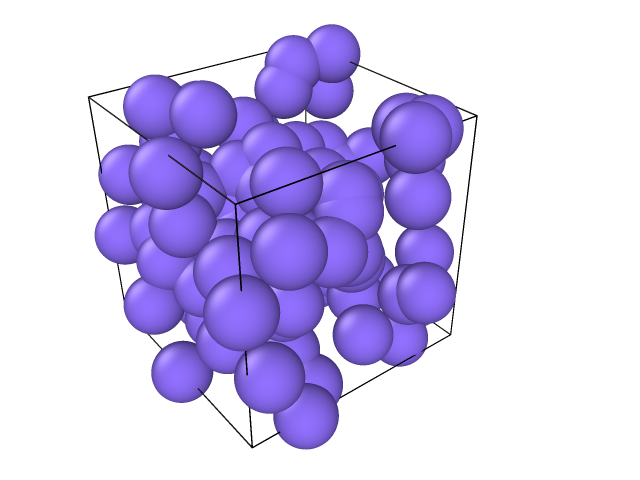
\includegraphics[width=\linewidth]{5cnoFCC.png}
  \caption{Tilfeldig plassering av atomer.}\label{fcuk}
\endminipage\hfill
\minipage{0.4\textwidth}
  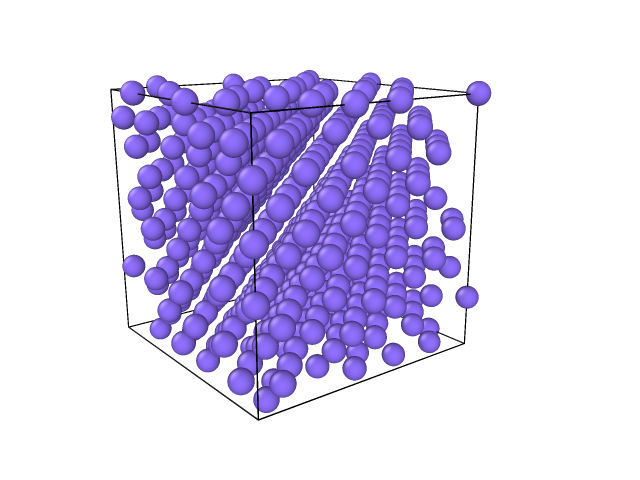
\includegraphics[width=\linewidth]{5cFCC.png}
  \caption{Atomer plassert i FCC gitterstruktur.}\label{fcuk2}
\endminipage\hfill
\end{figure}
 \FloatBarrier
 
Figur \ref{50}, \ref{250}, \ref{450} og \ref{700} viser hvordan systemet utviklet seg ved ulike initialtemperaturer på hvv 50, 250, 450 og 700 Kelvin. Her er det brukt 5$\times$5 $\times$ 5 enhetsceller, som tilsvarer 500 atomer. 
 
 
 \FloatBarrier
\begin{figure}[!htb]
\minipage{0.49\textwidth}
  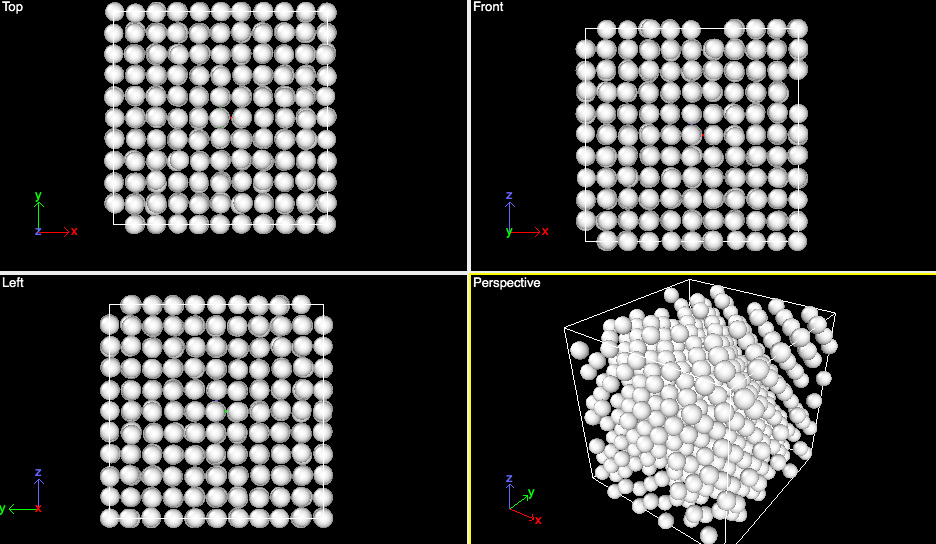
\includegraphics[width=\linewidth]{T=50}
  \caption{Initialtemperatur 50 K}\label{50}
\endminipage\hfill
\minipage{0.49\textwidth}
  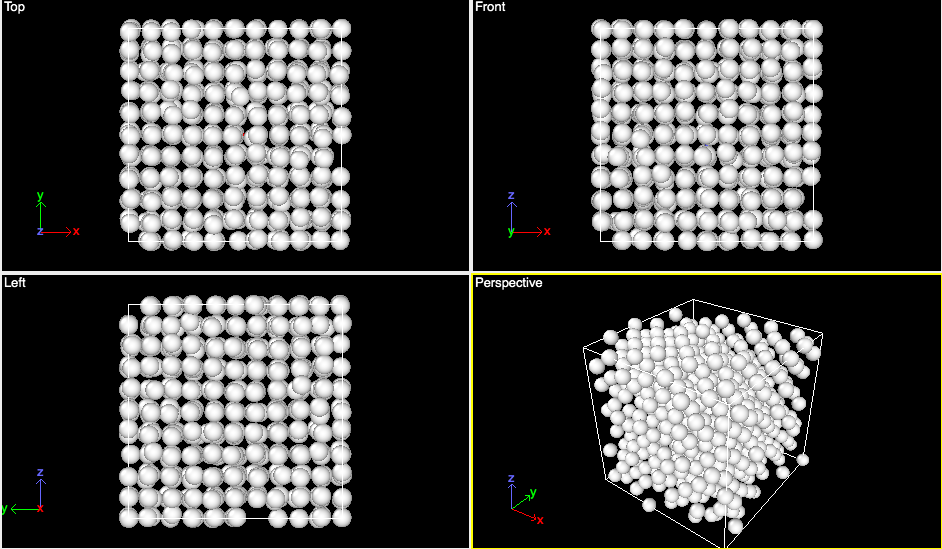
\includegraphics[width=\linewidth]{T=250}
  \caption{Initialtemperatur 250 K}\label{250}
\endminipage\hfill
\end{figure}
 \FloatBarrier
 
 \FloatBarrier
\begin{figure}[!htb]
\minipage{0.49\textwidth}
  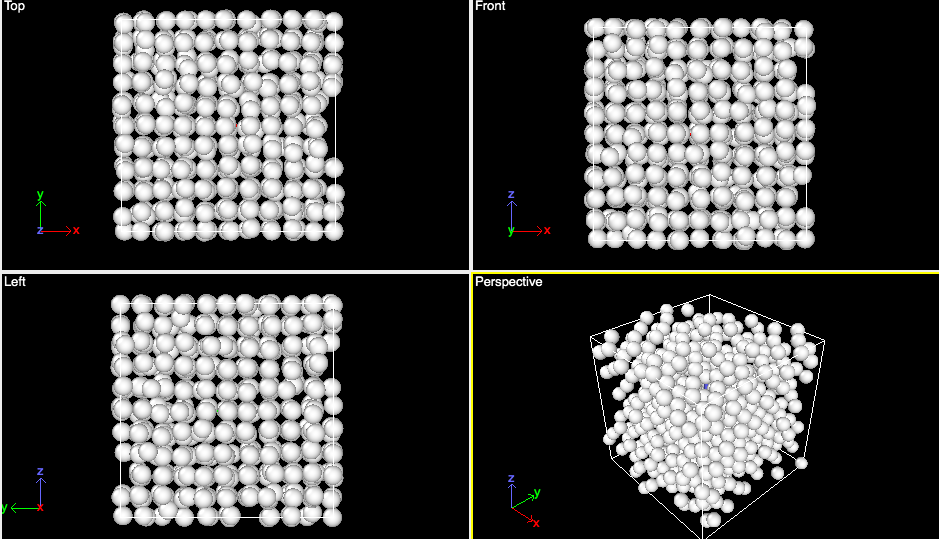
\includegraphics[width=\linewidth]{T=450}
  \caption{Initialtemperatur 450 K}\label{450}
\endminipage\hfill
\minipage{0.49\textwidth}
  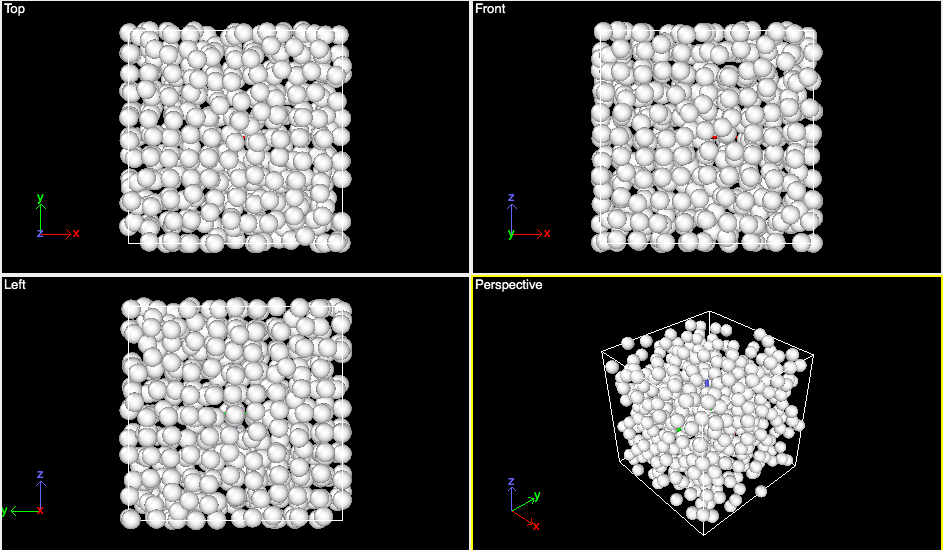
\includegraphics[width=\linewidth]{T=700}
  \caption{Initialtemperatur 700 K}\label{700}
\endminipage\hfill
\end{figure}
 \FloatBarrier

I figur \ref{TEMP} og \ref{Energy} ser vi hvordan temperaturen og energien utvikler seg som funksjon av antall tidssteg. 

 \FloatBarrier
\begin{figure}[!htb]
\centering
\minipage{0.5\textwidth}
  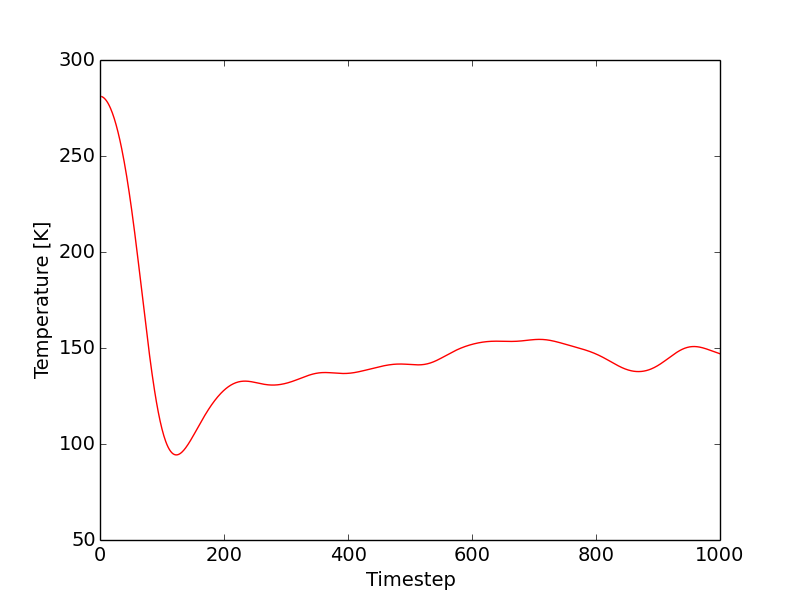
\includegraphics[width=\linewidth]{TvsStep.png}
  \caption{Temperatur som funksjon av antall tidssteg. Her er ett tidssteg det samme som $10^{-15}$ sekunder. }\label{TEMP}
\endminipage\hfill
\minipage{0.5\textwidth}
  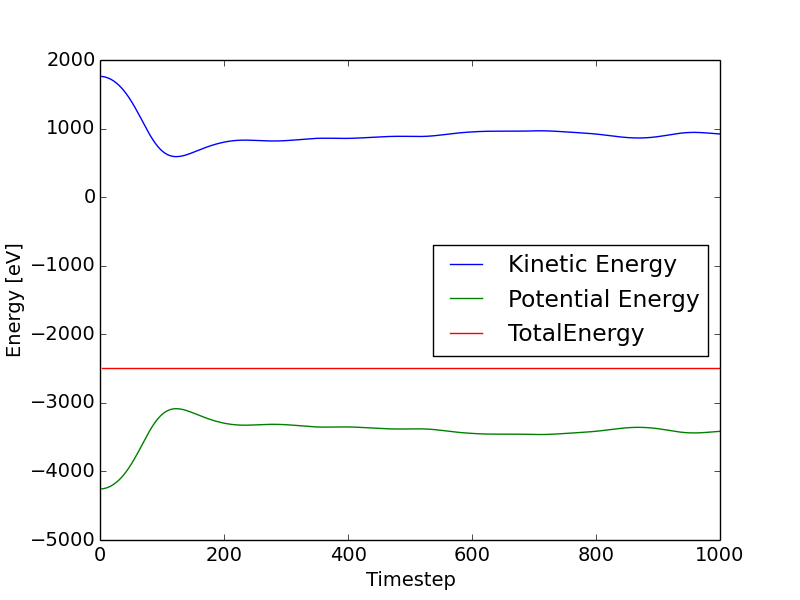
\includegraphics[width=\linewidth]{EvsStep.png}
  \caption{Potensiell, kinetisk og total energi som funksjon av antall tidssteg.}\label{Energy}
\endminipage\hfill
\end{figure}
 \FloatBarrier
 
I figuren under ser vi $T/T_{init}$ som funksjon av $T_{init}$, hvor $T$ er temperaturen til systemet etter det har nådd termisk likevekt, og $T_{init}$ er initialtemperaturen som systemet starter med.

\FloatBarrier
\begin{figure}[!ht]
 \centering
 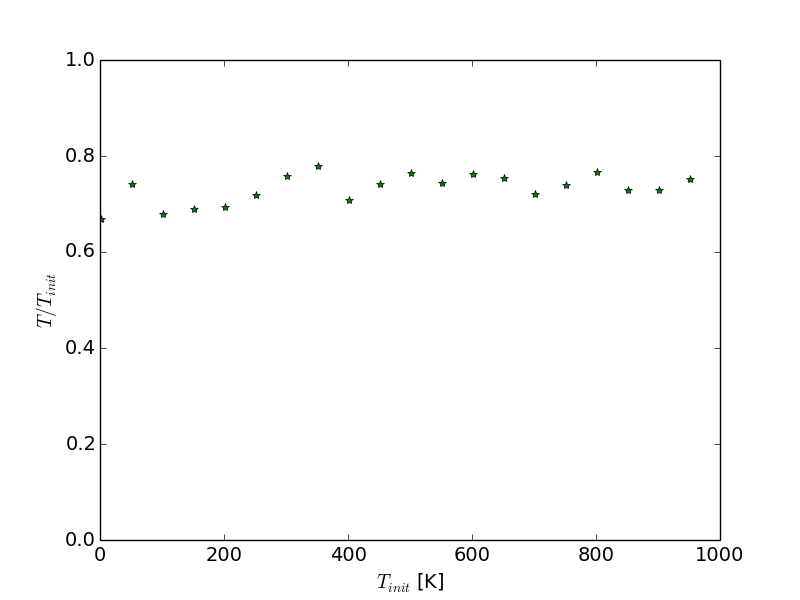
\includegraphics[scale=0.5]{T_ratio.png}
 \caption{Forholdet mellom temperatur og initialtemperatur som funksjon av initialtemperatur holder seg tilnærmet konstant.}
 \label{Trat}
 \end{figure}
 \FloatBarrier

\section{Diskusjon}
I figurene \ref{50}, \ref{250}, \ref{450} og \ref{700} ser vi hvordan systemet utvikler seg ved ulike initialtemperaturer. Som forventet, ser vi at  systemet blir mer kaotisk ved høyere initialtemperaturer. Ved såpass høye temperaturer (eks 700 Kelvin) vil ikke atomene være bundet til sin faste plass i krystallstrukturen, og systemet vårt blir flytende. Vi ser at ved en initialtemperatur på 50 K har vi fortsatt beholdt krystallstrukturen. Allerede ved en initialtemperatur på 250 K begynner det å bli vanskelig å se krystallstrukturen tydelig. Det ville være vanskelig å bestemme ved hvilken temperatur systemet vårt går over til å bli væske bare ved å se på disse bildene. Vi bruker derfor diffusjonskonstanten $D$ til å få et bedre estimat av smeltepunktet til systemet. \\

Temperaturutviklingen til systemet vises i figur \ref{TEMP}. Vi ser at systemet starter med en initialtemperatur på 300 K.  Graften starter med å synke brått i løpet av de første hundre tidsstegene. Vi vet at temperaturen er linket til atomenes kinetiske energi. Jo høyere kinetisk energi atomene har, jo høyere blir temperaturen. Vi ser i figur \ref{Energy} at også den kinetiske energien dropper i starten av simuleringen. Etter at temperaturen har droppet, stabiliserer temperaturen seg på omtrent halvparten av verdien til  initialtemperaturen. Det at temperaturen har stabilisert seg tyder på at systemet har nådd likevekt.\\

I figur \ref{Energy} ser vi kinetisk, potensiell og total energi i samme plott. Når vi så på verdien til totalenergien, oppdaget vi en liten fluktuasjon i det andre desimaltegnet. Dette kommer av avrundingsfeil og feil i Velocity Verlet integratoren. Vi kan derfor se bort fra disse fluktuasjonene. Den totale energien holder seg altså konstant, som forventet. Dette viser at koden vi har skrevet fungerer i henhold til de fysiske lovene. Den kinetiske energien faller også brått i starten, i likhet med temperaturen. Samtidig som den kinetiske energien faller, øker den potensielle energien. Det kommer av energibevaringen, da den totale energien må forbli konstant. Den hurtige økningen i potensiell energi kommer av at systemet mister sin krystallstruktur, hvor den potensielle energien er lavest. \\

Ved å simulere tidsutviklingen til systemet ved ulike initialtemperaturer $T_{init}$, kunne vi finne temperaturen $T$ ved termisk likevekt. I \ref{Trat} er forholdet $T/T_{init}$ plottet mot $T_{init}$. Dette folholdet holder seg nesten konstant ved 0.7. Dette viser at temperaturen ved likevekt er omtrent 70$\%$ av initialtemperaturen. For at systemet skal oppnå en endelig temperatur ved likevekt, spiller det altså ingen rolle hvilken initialtemperatur vi bruker, siden dette forholdet er konstant.\\




\section{Konklusjon}
I løpet av dette prosjektet har vi klart å implementere et program som bruker molekylærdynamikk til å simulere grunnstoffet Argon. Vi har sett på hvordan dette systemet oppfører seg ved ulike initialbetingelser. Ved å beregne ulike størrelser som potensiell energi, kinetisk energi, temperatur og diffusjonskonstant, kan vi se på hvordan disse vil utvikle seg som funksjon av tid. Vi har sett på gittere med størrelsen 5$\times$5$\times$5, og sett at koden fungerer ved hjelp av enkle tester som at den totale energien skal være bevart, og dermed konstant. 


\horrule{2pt} \\[0.5cm] % Thick bottom horizontal rule

\section{Appendix A}
I programmet vårt brukes det MD enheter, hvor de fire følgende enhetene er definert ved

\begin{align}
	\text{1 masseenhet } &= 1 \text{ atommasse } = 1.661\times 10^{-27}\mathrm{kg},\\
	\text{1 lengdeenhet } &= 1.0 \mathrm{angstrom} = 1.0\times 10^{-10}\mathrm{m},\\
	\text{1 energienhet } &= 1.651\times 10^{-21}\mathrm{J},\\
	\text{1 temperaturenhet} &= 119.735\mathrm{K}.
\end{align}

og vi får at Boltzmanns konstant $k_B$ = 1. Ut ifra dette kan vi utlede størrelsen på andre enheter, som for eksempel tid. Ved å bruke $E = mc^2$ får vi at
\begin{align}
\text{Energi} = \text{masse} \times \frac{\text{lengde}^2}{\text{tid}^2}
\end{align}

som gir oss 
\begin{align}
\text{Tid} = \text{lengde} \times \sqrt{\frac{\text{masse}}{\text{energi}}}
\end{align}

Setter vi inn de oppgitte verdiene for lengde, masse og energi, får vi at
\begin{align}
\text{1 tidsenhet } = 1.0 \times 10^{-10}\sqrt{\frac{1.661\times 10^{-27}}{1.651\times 10^{-21}}} \text{ s} = 1.00224\times 10^{-13}\mathrm{s}.
\end{align}

\horrule{2pt} \\[0.5cm] % Thick bottom horizontal rule
%----------------------------------------------------------------------------------------

\bibliography{Referanser}
\begin{thebibliography}{9}  
    
\bibitem{}
   M. Hjort-Jensen: Computational physics, lecture notes 2015. Fysisk institutt, UiO, 2016.

\bibitem{}
   Oppgavetekst: Project 5, Fysisk institutt, UiO, 19.11.16
   
\bibitem{}
 Gitterstrukturer: <http://frey.no/wp-content/uploads/2014/01/3-Gitterstrukturer.pdf>, 19.11.16  
 
 \bibitem{}
  Molekylærdynamikk: <https://no.wikipedia.org/wiki/Molekyl$æ$rdynamikk>, 19.11.16
  
\bibitem{}
 XYZ file formal: <https://en.wikipedia.org/wiki/XYZ$\_$file$\_$format>, 19.11.16
 
 \bibitem{}
 Opprinnelig kode, A. Hafreager: <https://github.com/andeplane/molecular-dynamics-fys3150>, 19.11.16
  
\bibitem{}
  Deler av koden er hentet fra: <https://github.com/GioPede/FYS3150/tree/master/Project5>,
  20.11.16
  
 \bibitem{}
 Periodic boundary conditions: <https://en.wikipedia.org/wiki/Periodic$\_$boundary$\_$conditions>, 20.11.16
 
 \bibitem{}
 van der Waals force: <https://en.wikipedia.org/wiki/Van$\_$der$\_$Waals$\_$force>

   
\end{thebibliography}

\end{document}